\section{Background}
In this section we dicuss

\subsection{Public-key Cryptography and Key Exchange}
Asymmetric cryptography facilitates the secure encryption of messages
in end-to-end encryption (E2EE), verification of digital signatures, and
sharing of pre-communication secrets, among others.

The asymmetry stems from the use of ``Public'' and ``Private'' keys. The
public-key is used to encrypt data that only the respective private-key
can decrypt. Hence, this means that sharing the keys required to encrypt
can be performed across insecure channels.

An E2EE connection uses the key types discussed previously to ex-
change messages between verified parties securely. However, this hinges
on the verification of the initial parties, if one party impersonates another and receives sensitive communication, the secure encryption is
completely circumvented. Therefore, the correct identification of parties is crucial to maintaining security. The exploitation of this is known as a Man-in-the-middle (MiTM) attack. This attack is commonly bidirectional, and if executed correctly, there is often no discerning change to the user experience.

\subsection{Similarity Metrics}
\label{sec:similarity_metric}
A similarity metric is an algorithm designed to determine if two words are phonetically a match. For example, the words "THEIR" and "THERE" is a match, whereas the words "DARK" and "PRINCIPLE" are not phonetically matching. This section provides a base explanation of important phonetic algorithms relevant in this project.

\subsubsection*{Soundex}
\label{sec:soundex}
One of the earliest examples of a phonetic algorithm is known as Soundex. It was initially designed for phonetically indexing names alongside detection of transposed letters in spelling mistakes.  Soundex is one of the most famous example of a phonetic. This is due in part to its implementation into major database clients like MySQL\cite{mysql_soundex}, Oracle\cite{moved_2005} and PostgreSQL\cite{postgresql}.

\subsubsection*{NYSIIS}
\label{sec:nysiis}
The New York State Identification and Intelligence System (NYSIIS) phonetic code was created for the phonetic matching of American names. The motivation for its inception was mostly due to the presence of Hispanic names in the American based databases (this was an aspect Soundex was known to have low accuracy with).

\subsubsection*{Metaphone}
\label{sec:metaphone}
Metaphone was invented by Lawrence Philips in 1990\cite{philips1990hanging} in response to the deficiencies in Soundex. It improves on Soundex by including information around inconsistency and variation in English spelling in an attempt to create a more accurate phonetic representation.

\subsubsection*{Levenshtein Distance}
\label{sec:leven}
Levenshtein distance is a string metric designed to measure the `distance' between two strings. It is merely the number of single-character edits (insertions, deletions or substitutions) required to reach the other string.

An example distance between \verb|trace| and \verb|place| would be the substitutions of the first to letters, from \verb|tr| to \verb|pl|, meaning the two strings have a Levenshtein distance of 2.

\subsubsection*{Phonetic Vectors}
\label{sec:phonetic_vectors}
Phonetic Vectors is a unique addition to the chosen set. Created by Allison Parrish in 2017\cite{parrish2017poetic}, Phonetic vectors is as the name suggests the vectorisation of the phonetics of a word. Phonetic features are used in this work as a way to compare the similarity of phonemes. Phonemes are the phonetic elements that construct a word. For example, the word "RING" translated into the phonemes \verb|/R IH NG/|. 

\clearpage

\subsection{Pretty Easy Privacy}
\label{sec:pep}
A very recent implementation of a word list can be found in Pretty Easy Privacy (\pep) implementation of TrustWords\cite{trustwords}. \pep is a data encryption system that utilises PGP encryption to provide E2EE on all common channels of communication such as email or SMS. The embedded design principles state that above all the systems should be easy to install, use and understand.

\pep deals with the threat of MiTM attacks by having users compare the respective key fingerprints encoded as a set of words. Figure \ref{fig:trustwords} shows the \pep Android implementation of Trustwords. The users then authenticate the words on an OOB (Out of Band) channel such as a phone call or in-person communication. If both users decide the words match, they accept or decline respectively.

\begin{figure}[h!]
    \centering
    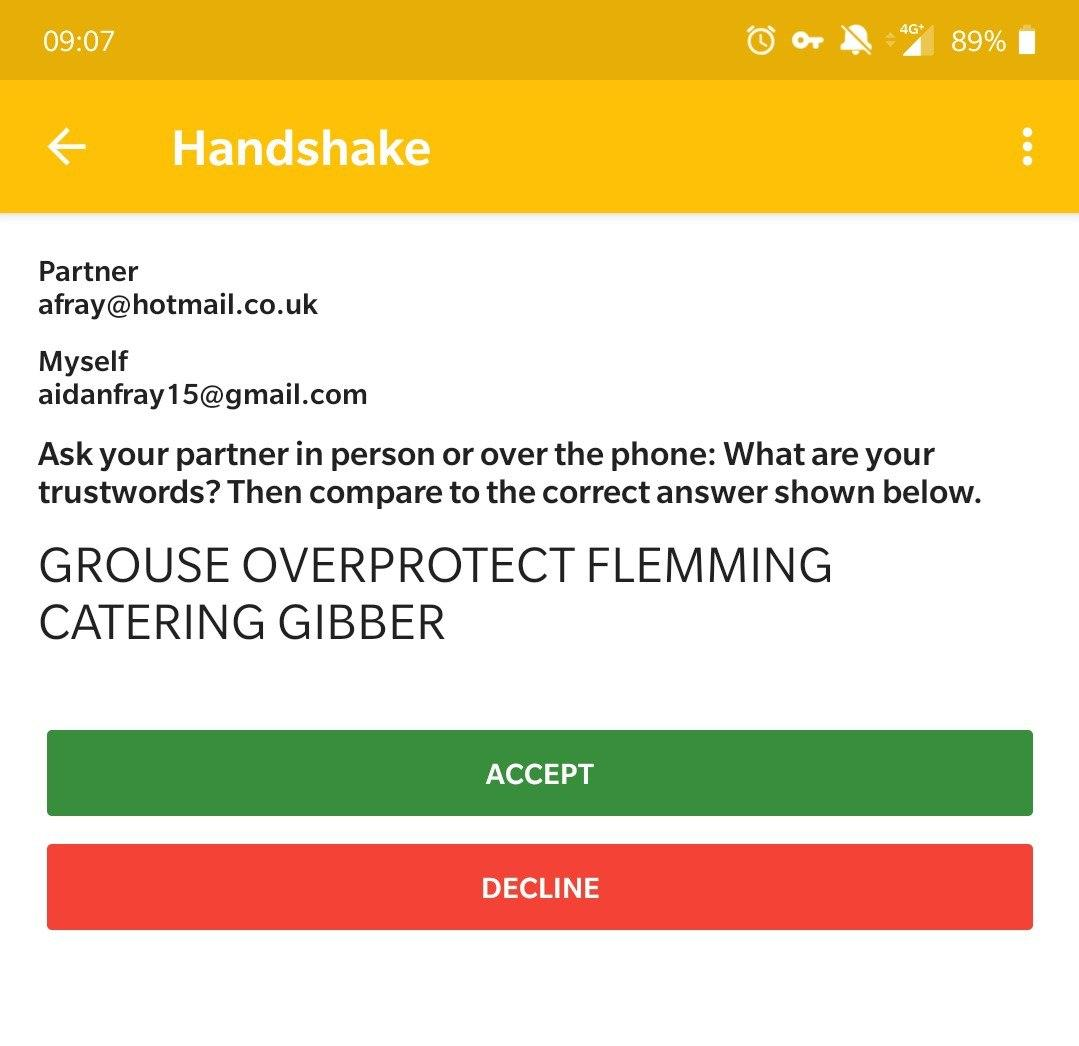
\includegraphics[width=0.4\textwidth]{trustwords/trustword_handshake.jpg}
    \caption{Trustword fingerprint verification}
    \label{fig:trustwords}
\end{figure}

The unique aspect of TrustWords is its mapping of a single word to 16-bits. If compared to alternative literature, this is the highest number of bits-per-word seen. Full mappings (no duplication of words) would, therefore, require $2^{16}$ words in the dictionary. This number of words is arguably higher than most users' vocabulary. This deviation from the norm has not been currently backed up by research. 
